\chapter{The DLS Method in Detail}

We now look at the mathematics behind the D/L, and DLS methods. D/L being the original
method, and DLS the method that Stern helped to revise. In the original paper, the authors
state ``Commercial confidentiality prevents the disclosure of the mathematical definitions
of these functions.'' $\cite{duckworth}$. Which is naturally a slight problem for this, but what
we can do is instead use sample values based on data we have to look at how these functions behave,
so all is certainly not lost.

\section{Origins: Duckworth and Lewis}
We begin by looking at the original paper. The first thing to establish is how many runs are scored,
on average, in a given number of overs. This is given by the equation:

\begin{equation}
    Z(u) = Z_0[1-exp(-bu)]
    \label{Z(u)}  
\end{equation}

Where u is the number of overs, b is the exponential decay constant, and $Z_0$ is the
average total score in first class cricket, but with one-day rules imposed.  

Now because we don't have access to actual values for $Z_0$ or b, a plot to see what equation \ref{Z(u)} looks 
like was created by using 3 sample values for $Z_0$. For b, it was a process of trial and error to find a value
that resulted in the graph having a similar shape to original figures in the D/L paper. 

\begin{figure}[h]
    \centering
    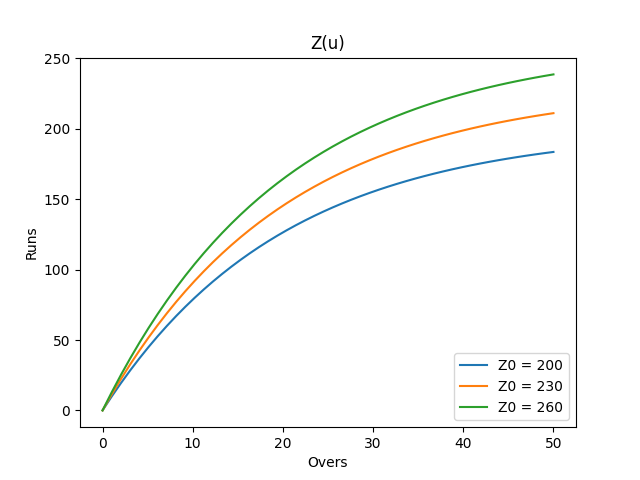
\includegraphics[scale=0.6]{figures/z(u).png}
    \label{Z(u)_graph}
    \caption{Graph showing how the rate at which runs are scored decays as a game progresses.}
\end{figure}

However, we have not yet looked at what happens when wickets are lost. To introduce this metric, equation \ref{Z(u)}
is revised to incorperate the scenario that w wickets have been lost, and that there are u overs remaining
The revised equation is given as follows:

\begin{equation}
    Z(u,w) = Z_0(w)[1-exp(-b(w)u)]
    \label{zuw}
\end{equation}

Where now, we have $Z_0(w)$ giving the average total score from the last $10-w$ wickets in first class cricket.
We now also have $b(w)$ as the exponential decay constant, which now changes depending on wickets lost.

With this in mind, we now look at the specific case of equation \ref{zuw} with $u=N$ and $w=0$, namely, the conditions
at the start of an N-over innings. We have:

\begin{equation}
    Z(N,0) = Z_0[1-exp(-bN)].
    \label{zstart}
\end{equation}

Which we then incorperate into the ratio

\begin{equation}
    P(u,w) = \frac{Z(u,w)}{Z(N,0)}.
    \label{prat}
\end{equation}

The ratio \ref{prat} gives, keeping in mind there are u overs still to be bowled, with w wickets
lost, the average proportion of the runs that still need to be scored in the innings. 
It is this ratio that is where the revised scores come from. Let us now look a bit more at how that works
practically.

\begin{example}
    \label{dlExMain}
    Assume there is a break in the second innings (due to rain or similar), which results in the second team missing some overs.
    Let $u_1, u_2$ be the number of overs played before the break, and available after it respectively. We impose the condition
    that $u_2 < u_1$. At the time of the break, the second team had lost $w$ wickets. The aim is to adjst the required score to account
    for the $u_1 - u_2$ overs they have lost. The winning ``resources'' available are given by

    \[
        R_2 = [1-P(u_1,w)+P(u_2,w)].
    \]  

    Which means, if the first team batting scored S runs, then the new tartget is given by

    \[
        T = \ceil{SR_2}
    \]  
\end{example}

\section{Improvements by Stern}
We now look at the DLS method, introduced by Stern in $\cite{stern}$ to extend the original D/L method. The motivation for DLS was that very high scoring
cricket matches presented a pattern of straightening towards average run rate which is not uniform across the innings considered (around 500). To account for 
this, Stern introduces an additional damping factor to the equation for D/L. The updated equation is now given by:

\begin{equation}
    \label{dls}
    Z_{dls}(u,w,\lambda) = Z_0F_w\lambda^{n_w+1} \left\{ 1-e^{-ubg(u,\lambda)/F_w\lambda^n_w} \right\}.
\end{equation}

This equation assumes u overs remaining, w wickets down in an M-over match with a final total of $S$. Here, we have:

\begin{equation}
    \label{gfunc}
    g(u,\lambda) = \left (\frac{u}{50} \right)^{-(1+\alpha_\lambda+\beta_\lambda u)}
\end{equation}

In the above, we define $a_\lambda = -1/\{1+c_1(\lambda-1)e^{-c_2(\lambda-1)}\}$ and $\beta_\lambda = -c_3(\lambda-1)e^{-c_4(\lambda-1)}$. The constants $c_1,\ldots,c_4$ are based on
what Stern describes as a ``detailed examination'' of high scoring cricket matches.

\section{Extension: Bayesian Modelling}
This section will look at the work of paper $\cite{dlbayes}$, which used Bayesian modelling to try and improve the score predictions
of the D/L method. The authors used the same dataset as we are using for the dissertation, although over a slightly smaller range of games.
Only games between 2005-2017 are used, whereas our dataset goes up to 2021. Note that to keep consistent with the fact we are talking about a different
model now, we swich from using $Z(u,w)$, to using $R(u,w)$, as to keep consistency with the different papers being looked at.
They start by introducing the following nonlinear regression model:

\begin{equation}
    \label{dlRegress}
    \bar{R}(u,w) \sim N(m(u,w;\theta),\frac{\sigma^2}{n_{uw}})
\end{equation}

Where $\bar{R}(u,w)$ is the sample average of runs scored by a team from the total number of matches in the data set. We have $m(u,w;\theta)$
as the corresponding modeled population average of runs scored by a team when a considerable amount of games are taken into account. $\theta$ denotes 
a vector of parameters that will be specified later on. Since $R(u,w)$ is not calculated in all games, the average score is taken over all matches where
scores are present, this is given by $n_{uw}$. The sample mean $\bar{R}(u,w)$ is the calculated over this quantity. This is actually the point which motivates
using Bayesian statistics to extend the D/L method. The authors report that approximately $26.8\%$ of values for $R(u,w)$ were missing in the dataset, so by 
using a Bayesian inference model, we can use the posterior predictive distribution to account for missing values. Which in turn should increase the 
predictive accuracy of this model. \\

We return now to look at the $m(u,w;\theta)$ parameter that appears in \ref{dlRegress}. This mean function, based on the plots produced in the original D/L
paper, (see \ref{Z(u)_graph} for an example), the authors adopted an exponential decay. We can see why this choice makes sense from figure \ref{Z(u)_graph}.
The resources considered by this method, namely runs and wickets, do decrease exponentially as a game progresses. $m(u,w;\theta)$ depends on the parameters
$a_w = Z_0(w)$ and $b_w = b(w)$, each one depending on the number of wickets fallen at that given time, with u overs remaining. We therefore have:

\begin{align}
    \label{mdef}
        m(u,w;\theta) &= a_w(1-exp(-b_wu)) \\
               \theta &= \{ (a_w,b_w); w \in \mathcal{W}=\{0,1,\ldots,9\} \} 
\end{align}

Before proceeding with defining the prior specifications on the parameters for this model, we need the following distribution:

\begin{definition}
    $X \sim Ga(a,b)$ has a \textbf{Gamma Distribution} with mean $\frac{a}{b}$ and variance $\frac{a}{b^2}$ if its probability density function is
    $$
        \frac{b^a}{\Gamma(a)} x^{a-1}e^{-bx}.  
    $$
\end{definition}

We can now define the prior specifications on the parameters. First, we fix $A_0$ and $B_0$ large enough such that $R(50,0) < A_0$. We initialise  the model with
$a_0 \sim U(0,A_0)$ and $b_0 \sim U(0,B_0)$. Then given any pair $(a_0,b_0)$ and for $w=0,1,\ldots,8$, we generate:

\begin{align}
    a_{w+1}|\sigma^2,a_w,b_w &\sim U(0,a_w) \\
    b_{w+1}|\sigma^2,a_{w+1},b_w,a_w &\sim U\left(0,\frac{a_wb_w}{a_{w+1}}\right) \\
    \frac{1}{\sigma^2} &\sim Ga(a,b).
\end{align}

Above, U(a,b) represents a uniform distribution over the open interval $(a,b)$. Now that the prior distribution is obtained, the likelehood function is then 
given by:

\begin{equation}
    L(\theta,\sigma^2) = \left( \frac{1}{\sigma / \sqrt{n_{uw}}} \right)^{500} exp \left\{ - \frac{1}{2(\sigma^2 / n_{uw})} \sum_{u=1}^{50} \sum_{w=0}^9 (R(u,w)-m(u,a_w,b_w))^2  \right\}
\end{equation}

The authors chose their parameters $A_0, \ B_0, \ a \ \text{and} \ b$ such that the prior is not sensitive to the posterior inderence. The values chosen
were therefore $A_0=200 \ B_0=100 \ \text{and} \ a=b=0.1$.

One thing briefly mentioned in chapter 3 of this paper is the average score at the fall of each wicket. This isn't discussed further, but it's interesting to see how it behaves.
So we take a brief detour to look at it. This can be seen in figure \ref{avgrunsfow}.

\begin{figure}[h]
    \centering
    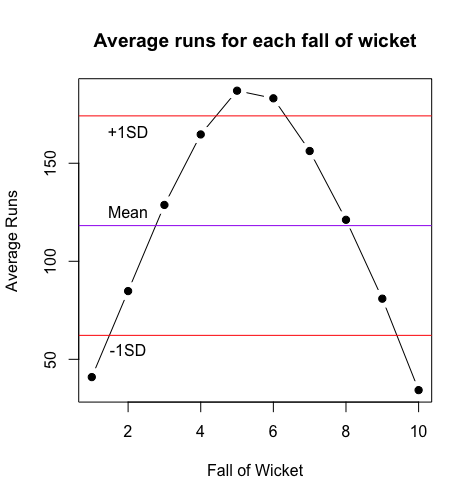
\includegraphics[scale=0.6]{figures/avgrunsfow.png}
    \caption{Plot of average runs scored at the fall of each wicket. Averages taken over 1437 innings.}
    \label{avgrunsfow}
\end{figure}
%NEED APPENDIX TALKING ABOUT KOLMOGROV-SMIRNOV
Initially, one may think that this is normally distributed. It certainly holds a bell curve-like shape. However, a Kolmogorov-Smirnov test $\cite{kolm}$ was
performed to see if these values were normally distributed, and it turns out they aren't. This test was performed using the R function \textit{ks.test()}, which returned
a p-value of $2.2\text{x}10^{-16}$ for the two-sided alternative hypothesis parameter. \\

Does the shape of this curve make sense? Well yes, because usually batters 3/4 are actually the best in the side, so the fact they put on more runs is not a suprise.
But what this does do is reinforce the idea behind using an exponential decay for modelling resources. This is because cumulatively, the tail end of batters (the last 4) 
will not put on as many runs as the higher/middle order. \\

Most of the work from this paper went into creating a better resource table for calculating revised scores. Which isn't particularly relevant to this project, but what is 
is the section on score prediction. The authors split every match at the $35^{th}$ over to try and predict the final score. They found the bayesian model gives a better
prediction of final match scores. Figure 3 of their paper outlines these results.